\label{sec:drahtlosedatenübertragung}
Drahtlose Datenübertragungverfahren ermöglichen die Übertragung von Informationen ohne elektrische Leiter. Sie nutzen elektromagnetische Wellen (Radiowellen), Magenetelder und elektrische Felder als Übertragungsmedium und können somit eine Kommunikation über Entfernungen von mehreren Kilometern oder mehr ermöglichen. 

Dieses Grundlegende Prinzip ermöglicht Anwendungen die deutlich portabler und flexiebler sind als kabelgebunden Verbindungen. Der Kernmechanismuss besteht darin die am Sender als elektrisches Signal Vorliegenden Daten in elektromagnetische Wellen umzuwandeln die sich dann durch die Umgebung ausbreiten können. Diese Signale können dann beim Empfänger wiederum in elektrische Signale umgewandelt und somit interpretiert werden. 

Für die drahtlose Telekommunikation werden überweigend elektromagnetische Wellen, insbesondere Funkwellen, eingesetzt. Drahtlose Kommunikationssysteme arbeiten in verschiedenen Frequenzbändern, die stark reguliert sind, um mögliche Interferenzen zu vermeiden. \autocite{GrundkenntnisseDrahtlosenKommunikation2023} 

Bekannte Modulationsverfahren lassen sich in Analoge und Digitale Verfahren aufteilen. Bei der analogen Modulation werden die Parameter des Trägersignals (Amplitude Modulation (AM) oder Frequenz Modulation (FM)) kontinuierlich entsprechend dem analogen Eingangssignal verändert. Bei der digitalen Modulation hingegen wird zwischen diskreten, fest definierten Zuständen umgeschaltet, um digitale Daten zu übertragen. \autocite[S. 112 ff. und S. 156 ff.]{ziemerPrinciplesCommunicationsSystems2015}

Ein einfaches Digitales Übertragungsprotokoll ist hier bei das Frequency Shift Keying (FSK), dabei werden digiale informationen durch die Variation der Frequenzen eines Trrägers kodiert. Im Wesentlichen wird die Trägerfrequenz periodisch zwischen mehreren Frequenzen verschoben, wobei jede Frequenz ein bestimmtes digitales Symbol darstellt.

Das einfachste FSK-Verfahren ist die binäre FSK (Binary FSK, BFSK oder 2-FSK), bei der zwei unterschiedliche Frequenzen verwendet werden, um die Binärziffern '0' und '1' zu repräsentieren. Wie in Beispielsweise Abbildung \ref{fig:frequency-shift-keying} kann eine höhere Frequenz eine binäre '1' darstellen, während eine niedrigere Frequenz eine binäre '0' repräsentiert. Wenn die zu übertragenden Daten eine '0' enthalten, wird die Trägerfrequenz $t_1$ verwendet um dieses Bit zu übertragen, wenn die Daten eine '1' sind, wird die Trägerfrequenz $t_2$ verwendet.\autocite{FrequencyShiftKeyingModulation2024}

\begin{figure}[H]
\centering
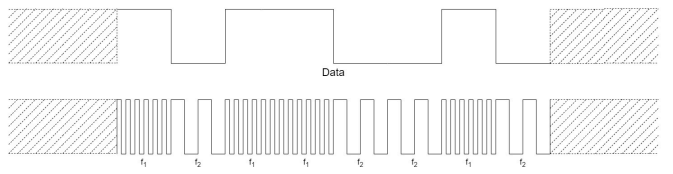
\includegraphics[scale=.5]{figures/asstes/frequency-shift-keying.png}
\caption{Frequency Shift Keying | Quelle: \autocite {FrequencyShiftKeyingModulation2024}}
\label{fig:frequency-shift-keying}
\end{figure}